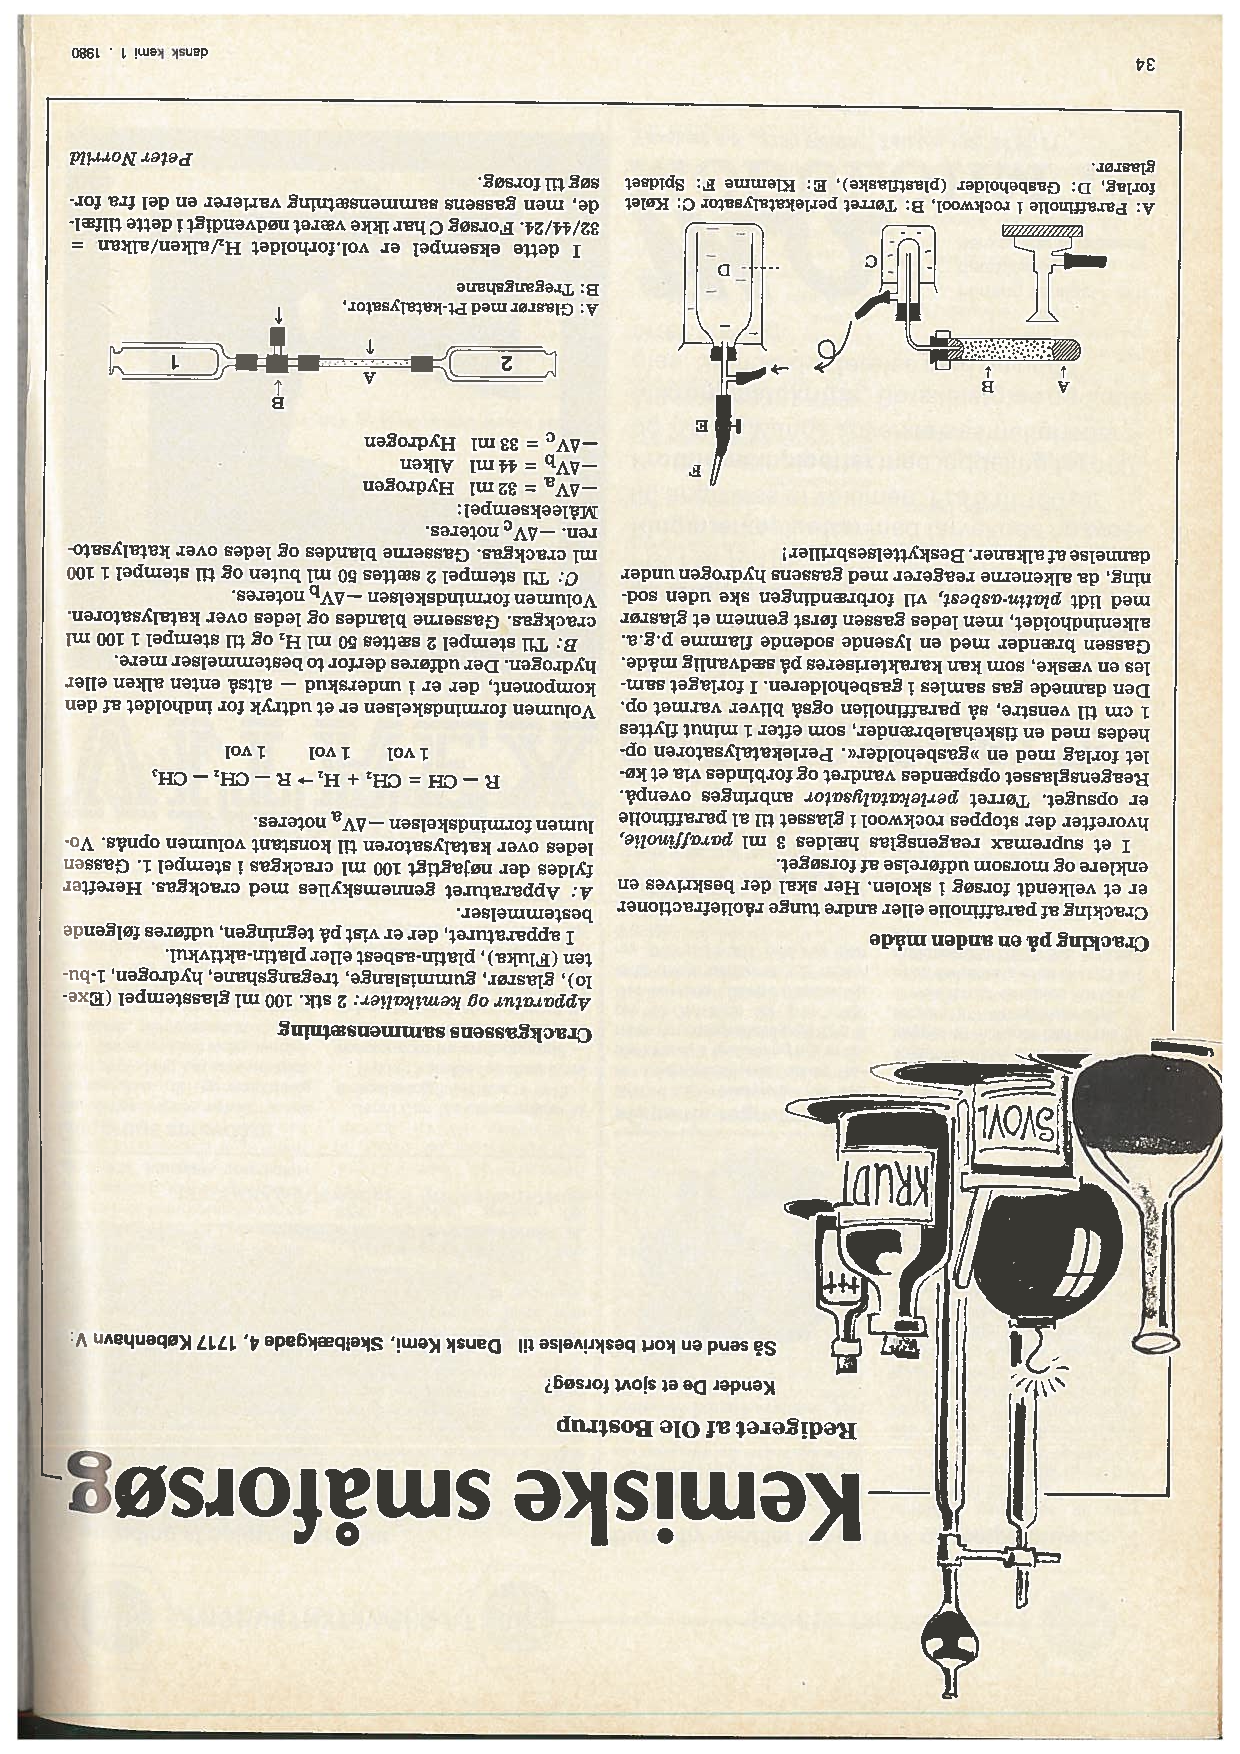
\includepdf[pages=-]{pdfs/1980-61-1-34.pdf}
Cracking på en anden måde
dansk kemi vol 61 iss 1 p 34



Forfatter:

Cracking af paraffinolie eller andre tunge råoliefractioner er et velkendt
forsøg i skolen. Her skal der beskrives en enklere og morsom udførelse af
forsøget.

I et supremax reagensglas hældes 3 ml paraffinolie, hvorefter der stoppes
rockwool i glasset til al paraffinolie er opsuget. Tørret perlekatalysator
anbringes ovenpå. reagensglasset opspændes vandret og forbindes via et kølet
forlag med en "gasbeholder". perlekatalysatoren ophedes med en fiskehalebrænder,
som efter 1 minut flyttes 1 cm til venstre, så paraffinolien også bliver varmet
op. Den dannede gas samles i gasbeholderen. I forlaget samles en væske, som kan
karakteriseres på sædvanlig måde. Gassen brænder med en lysende sodende flamme
p.g.a. alkenindholdet, men ledes gassen først gennem et glasrør med lidt
platin-asbest, vil forbrændingen ske uden sodning, da alkenerne reagerer med
gassens hydrogen under dannelse af alkaner. Beskyttelsesbriller!

Crackgassens sammensætning

Apparatur og kemikalier: 2 stk. 100 ml glasstempel ()
